\chapter{RQ2: Growing families from a seed}
\label{ch:rq2}

\begin{instructions}
About 4 pages. Answers RQ2, the plan's RQ2, and carries the plan's RQ3 scale pilot. Sources:
\src{docs/rq_roundA/RQ2-exemplar-seeded-search.md}, \src{docs/rq_roundA_2/RQ2b-second-seed.md}, and
\src{docs/rq_roundA_2/findings/rq2-blind-2026-10-26.md} (the surrogate table now; the blind panel's scores once queue
35 is judged and scored with \src{scripts/rq2_blind.py}). The scale pilot is
\src{docs/rq_roundA/RQ3-identity-under-scale.md}.
\end{instructions}

\section{Aims}

RQ2 asks whether a human-checked motif from the library, used as a seed, finds new instances that a human judging blind also accepts. Those instances must be accepted more often than duration-matched random windows, and must be far more numerous than the same search finds in a surrogate. If a researcher cannot retrieve more of a shape by querying with one example of it, the library has no way to grow except by hand.

\section{Methods}

\begin{instructions}
Cover:
\begin{itemize}
  \item \textbf{Seeds.} Medoids of Library families on M2\_aug. Dip id010 (family 24, 105\,s, CH4\_A2); long dip id020
        (family 23, 816\,s, CH1\_A1); spike (entry 289, family 37, 148\,s, CH1\_A1 at 248.4\,h); drop30 (family 30,
        entry 185, 377\,s); trough id022 (family 166, 327\,s).
  \item \textbf{Search.} The $d_z$ distance profile against every channel over 721\,h; $k=200$ matches per channel,
        exclusion zone $m/2$; 200 phase-randomised null draws per channel; the null's recommended cut. Searches longer
        than about 10 minutes ran as SLURM jobs on rangpur and were imported (\src{scripts/seed_job_parallel.py}).
  \item \textbf{Judging.}
        \begin{itemize}
          \item unblinded first: you knew each item was a match;
          \item then the blind panel, queue 35, 249 items shuffled with nothing showing their source: 100 drop30
                matches, 29 spike37 matches, 20 + 20 previously accepted dips judged again, and 80 random windows
                matched to the seeds' lengths (40 / 16 / 12 / 12 at 377 / 148 / 105 / 816\,s) on the same channels;
          \item items already judged as human spans were excluded from every pool alike.
        \end{itemize}
  \item \textbf{Scoring.} Acceptance per source with Wilson intervals; each seed against its duration-matched controls
        (Newcombe difference, Fisher's exact test); blind against unblinded agreement on the re-judged dips (Cohen's
        $\kappa$).
\end{itemize}
\end{instructions}

\section{Results}

\begin{figure}[htbp]
\centering
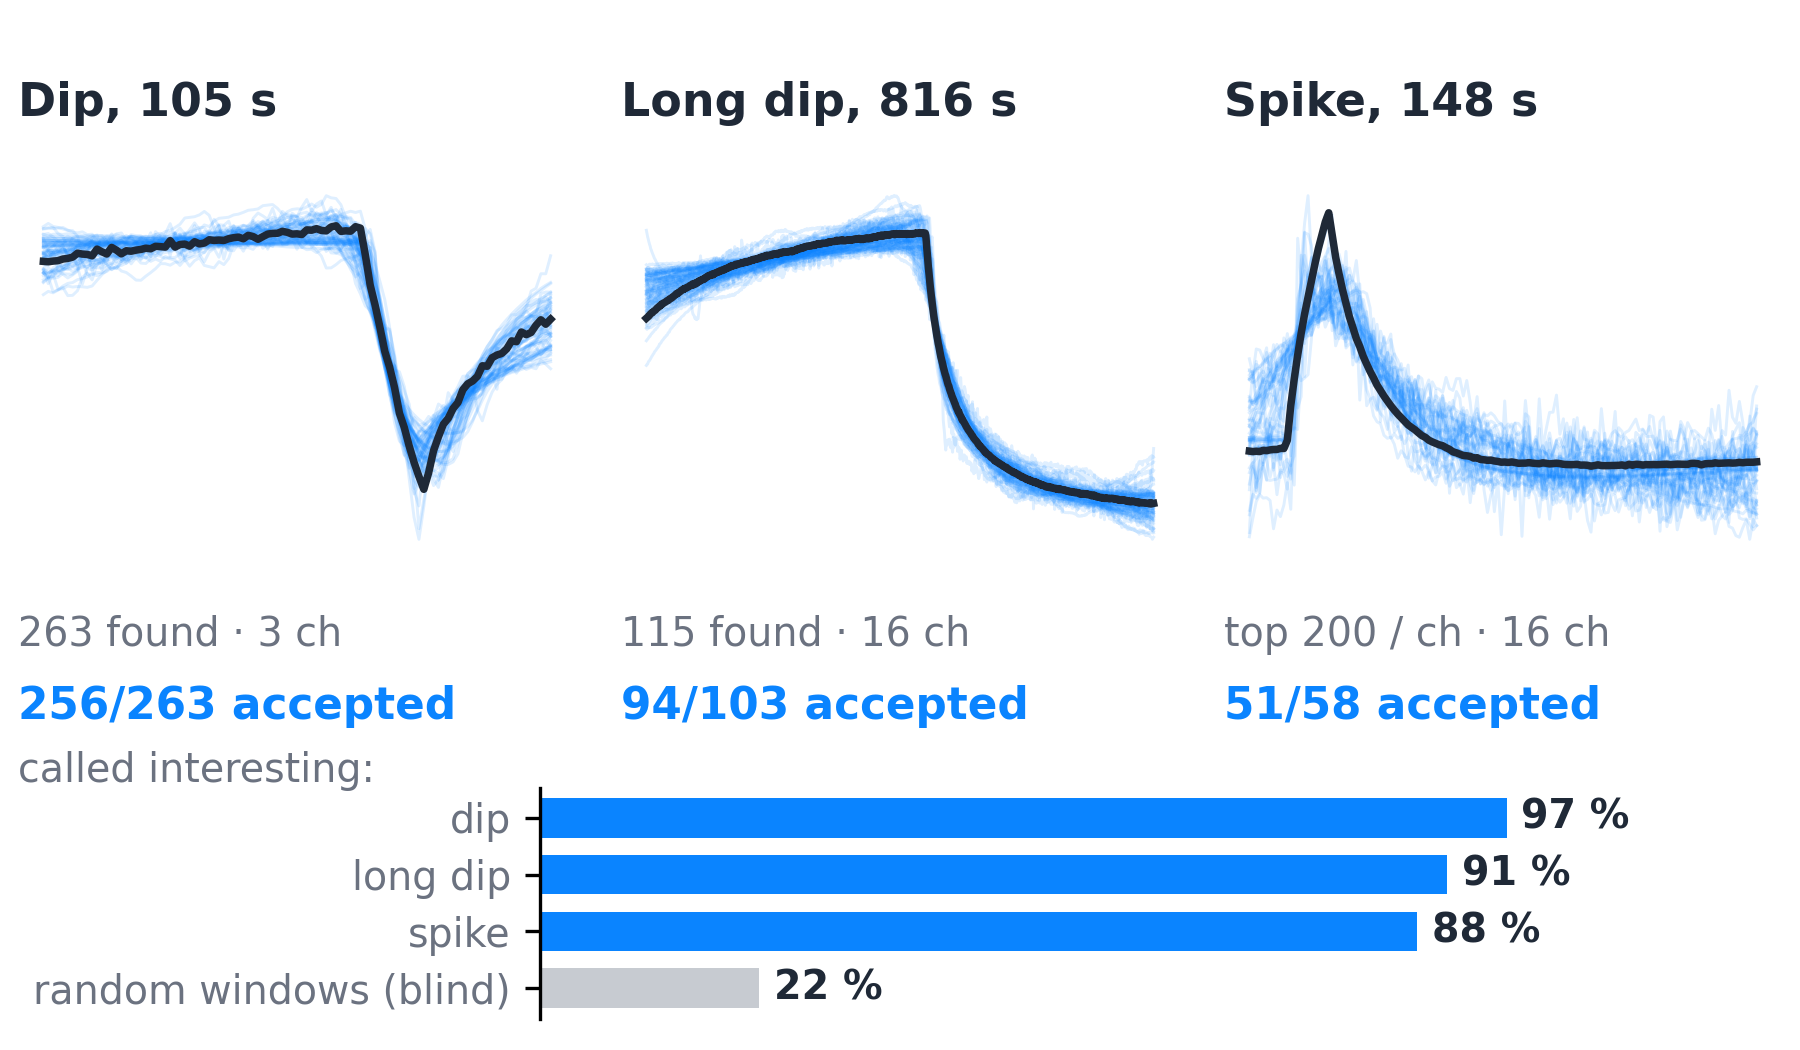
\includegraphics[width=0.9\textwidth]{poster/rq2_seeds.png}
\caption{Three seeds and their accepted matches overlaid (unblinded judging), with the share called interesting against random windows judged blind. From the poster; to be redrawn with the blind panel's results.}
\label{fig:seeds}
\end{figure}

\begin{table}[htbp]
\caption{Seed searches: matches under the null's cut against surrogate matches at the same threshold, and human acceptance. Unblinded figures from the earlier queues; blind figures from queue 35.}
\label{tab:seeds}
\footnotesize
\begin{tabularx}{\textwidth}{l r r r r r X}
\toprule
\textbf{Seed} & \textbf{Length} & \textbf{Ch} & \textbf{Matches} & \textbf{Null/draw} & \textbf{Unblinded} & \textbf{Blind (queue 35)}\\
\midrule
Dip id010 & 105\,s & 3 & 64 (263 at cut 2.652) & 0.01 (0.8) & 256/263 (97\,\%) & [re-judge 20]\\
Long dip id020 & 816\,s & 16 & 124 & 0.04 & 94/103 (91\,\%) & [re-judge 20]\\
Spike (entry 289) & 148\,s & 16 & 16 & 0.00 & 51/58 (88\,\%) & [29]\\
Drop30 (entry 185) & 377\,s & 16 & 372 & 0.01 & -- & [100]\\
Random windows & matched & -- & -- & -- & 235/1,084 (22\,\%) & [80 controls]\\
\bottomrule
\end{tabularx}
\end{table}

\begin{instructions}
Unblinded rates exclude \texttt{unsure} and \texttt{artifact} verdicts, as everywhere else in the thesis: id020's
94/103 leaves out 1 unsure, and the spike's 51/58 leaves out 2 unsure and 1 artifact (51/59 = 86\,\% if artifact counts
as ``not''). Fill the blind column after scoring. The test RQ2 needs is each seed's blind acceptance against its own
duration-matched controls, not against the earlier 22\,\% from a different queue. The re-judged dips tell you how much
knowing the source inflated the unblinded rates.

Report the surrogate side as it stands. Across seeds, scrambled copies of the signal give about zero matches per draw
at each seed's cut, against 16--372 real matches. On CH2\_A1, 60 of drop30's 65 family members are among its matches.

Caveats:
\begin{itemize}
  \item $k=200$ caps the count on busy channels (CH2 already at 111);
  \item only phase randomisation was used;
  \item all seeds and matches are within one experiment (M2\_aug).
\end{itemize}
Use the per-run report figures (\src{figures/reports/dip_null.png}, \src{figures/reports/spike_null.png}) for the null
histograms.
\end{instructions}

\begin{figure}[htbp]
\centering
\begin{subfigure}{0.49\textwidth}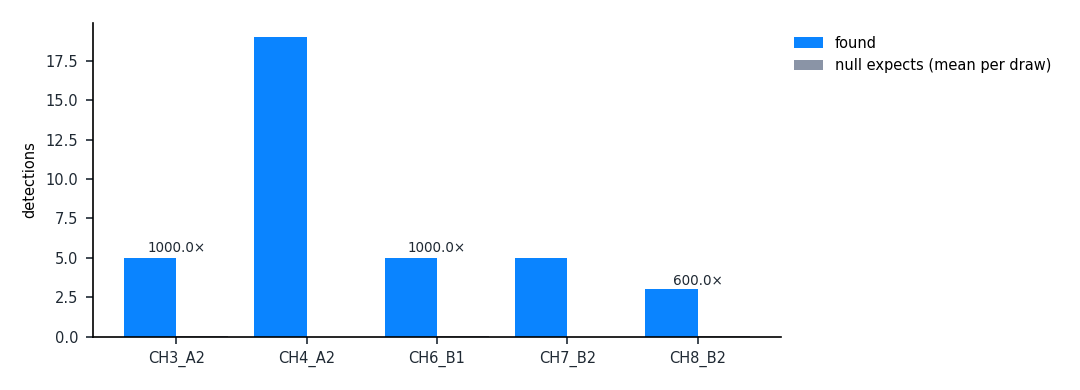
\includegraphics[width=\linewidth]{reports/dip_null.png}\caption{Dip seed}\end{subfigure}\hfill
\begin{subfigure}{0.49\textwidth}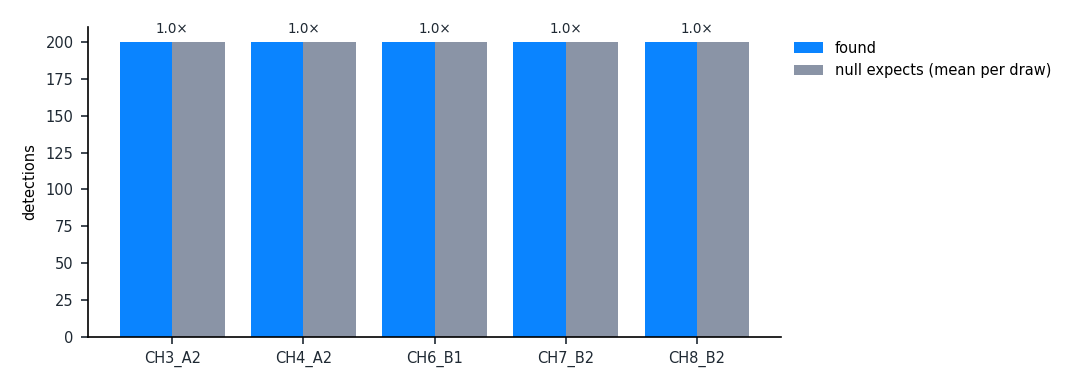
\includegraphics[width=\linewidth]{reports/spike_null.png}\caption{Spike seed}\end{subfigure}
\caption{Match distances per channel against the 200-draw phase-randomised null, with the cut each report recommends.}
\label{fig:seednull}
\end{figure}

\subsection{The scale pilot}

\begin{instructions}
The plan's RQ3 (does identity survive scale normalisation?) reduced to a pilot:
\begin{itemize}
  \item banked searches at 0.8$\times$, 1$\times$ and 1.25$\times$ the native length; so far only placeholder verdicts
        (an agent rule, $d<2$ accepted);
  \item for exemplar E-0697 at 0.8$\times$, the scale-invariant distance is 0.96 / 1.43 against 11.8 / 11.9 for the
        native-length control;
  \item the null at 0.8$\times$ gives about twice the matches of 1$\times$ (16.7 against 8.4 per draw);
  \item family F-130 holds together only after stretching: MPdist 0.68 (noise level) against scale-invariant 0.13.
\end{itemize}
If round B judges the banked searches, report recovery against duration here. Otherwise say plainly that RQ3 is a
pilot, and point to Chapter~\ref{ch:events} for the stronger evidence about scale.
\end{instructions}

\section{Discussion}

\begin{instructions}
Points to argue:
\begin{itemize}
  \item Seed search is how the library grows: one checked shape yields hundreds of candidates, at a known rate above
        chance.
  \item How much unblinded judging inflated the rates (from the re-judges).
  \item Matches per hour as a prevalence measure: what the matrix profile says about how common a motif is.
  \item What remains: cross-recording seeds (an M2\_aug seed on lion's mane, say), and seeds at other scales.
\end{itemize}
\end{instructions}
